\documentclass[11pt]{article}
\usepackage{latexsym}
\usepackage{amsmath}
\usepackage{amssymb}
\usepackage{amsthm}
\usepackage{epsfig}
\usepackage[tight]{subfigure}
\usepackage{hyperref}
\usepackage{listings}
\usepackage{xcolor}

\usepackage{amsmath}

\DeclareMathOperator*{\minimize}{min}
\DeclareMathOperator*{\maximize}{max}

\usepackage{algorithm}
 %on linux you may need to run sudo apt-get install texlive-full to install algorithm.sys
\usepackage{algorithmic}

\usepackage{verbatim}

\newcommand{\handout}[5]{
  \noindent
  \begin{center}
  \framebox{
    \vbox{
      \hbox to 5.78in { {#1} \hfill #2 }
      \vspace{4mm}
      \hbox to 5.78in { {\Large \hfill #5  \hfill} }
      \vspace{2mm}
      \hbox to 5.78in { {\em #3 \hfill #4} }
    }
  }
  \end{center}
  \vspace*{4mm}
}

\newcommand{\lecture}[5]{\handout{#1}{#2}{#3}{#4}{#5}}
\newcommand{\collision}[0]{\mathrm{collision}}
\newcommand{\nocollision}[0]{\overline{\collision}}

\newcommand*{\QED}{\hfill\ensuremath{\square}}

\newtheorem{theorem}{Theorem}
\newtheorem{corollary}[theorem]{Corollary}
\newtheorem{lemma}[theorem]{Lemma}
\newtheorem{observation}[theorem]{Observation}
\newtheorem{proposition}[theorem]{Proposition}
\newtheorem{definition}[theorem]{Definition}
\newtheorem{claim}[theorem]{Claim}
\newtheorem{fact}[theorem]{Fact}
\newtheorem{assumption}[theorem]{Assumption}
\newtheorem{note}[theorem]{Note}

% 1-inch margins, from fullpage.sty by H.Partl, Version 2, Dec. 15, 1988.
\topmargin 0pt
\advance \topmargin by -\headheight
\advance \topmargin by -\headsep
\textheight 8.9in
\oddsidemargin 0pt
\evensidemargin \oddsidemargin
\marginparwidth 0.5in
\textwidth 6.5in

\parindent 0in
\parskip 1.5ex
%\renewcommand{\baselinestretch}{1.25}

\begin{document}

\lecture{Statistical Techniques in Robotics (16-831, S22)}{Lecture \#20
  (Monday, April 4)}{Lecturer: Kris Kitani}{Scribes: Young Woo Kim, Dakshit Agrawal}{Function Approximators for Control, Policy Gradient Methods}

\section{Review}

%This section serves as a review of the previous lecture and any other context required to frame the content of the current lecture. 

%You may format the scribes in any way you like, aside from changing font style, size and page format. Please use subsections and paragraphs to increase the readability of your notes.

%Length requirement 1-2 pages.

% \subsection{General overview of what we have learned till now (value-based methods figure)}

In the past few lectures, we have learned many RL approaches (see Fig. \ref{fig:model-free}) for environments where we don't have access to the reward function $R(s^{(t)}, a^{(t)})$ and the transition function $p(s^{(t+1)}|s^{(t)}, a^{(t)})$, also known as model-free environments. The general idea is to sample ($s^{(t)}, a^{(t)}, r^{(t)}, s^{(t+1)}$) from the environment using the behavior policy $\mu(a^{(t)}| s^{(t)})$.  These approaches can be used for:
\begin{itemize}
    \item \textbf{Prediction} of the expected total rewards when at a state $s^{(t)}$ (value function $V(s^{(t)})$) or when at a state $s^{(t)}$ and taking an action $a^{(t)}$ (state-value function $Q(s^{(t)}, a^{(t)})$).
    \item \textbf{Control} by learning the target policy $\pi(a^{(t)}| s^{(t)})$ to maximize rewards in the model-free environment.
\end{itemize}

The approaches we have learned can alternatively be classified into the following types:

\begin{itemize}
    \item \textbf{On-Policy:} the behavior policy $\mu$ is the same as the target policy $\pi$, i.e., we sample from the environment using the same policy for which we are estimating the value function.
    \item \textbf{Off-Policy:} the behavior policy $\mu$ is different from the target policy $\pi$, i.e., we use someone else's experience to sample from the environment.
\end{itemize}


\begin{figure}[H]
    \centering
    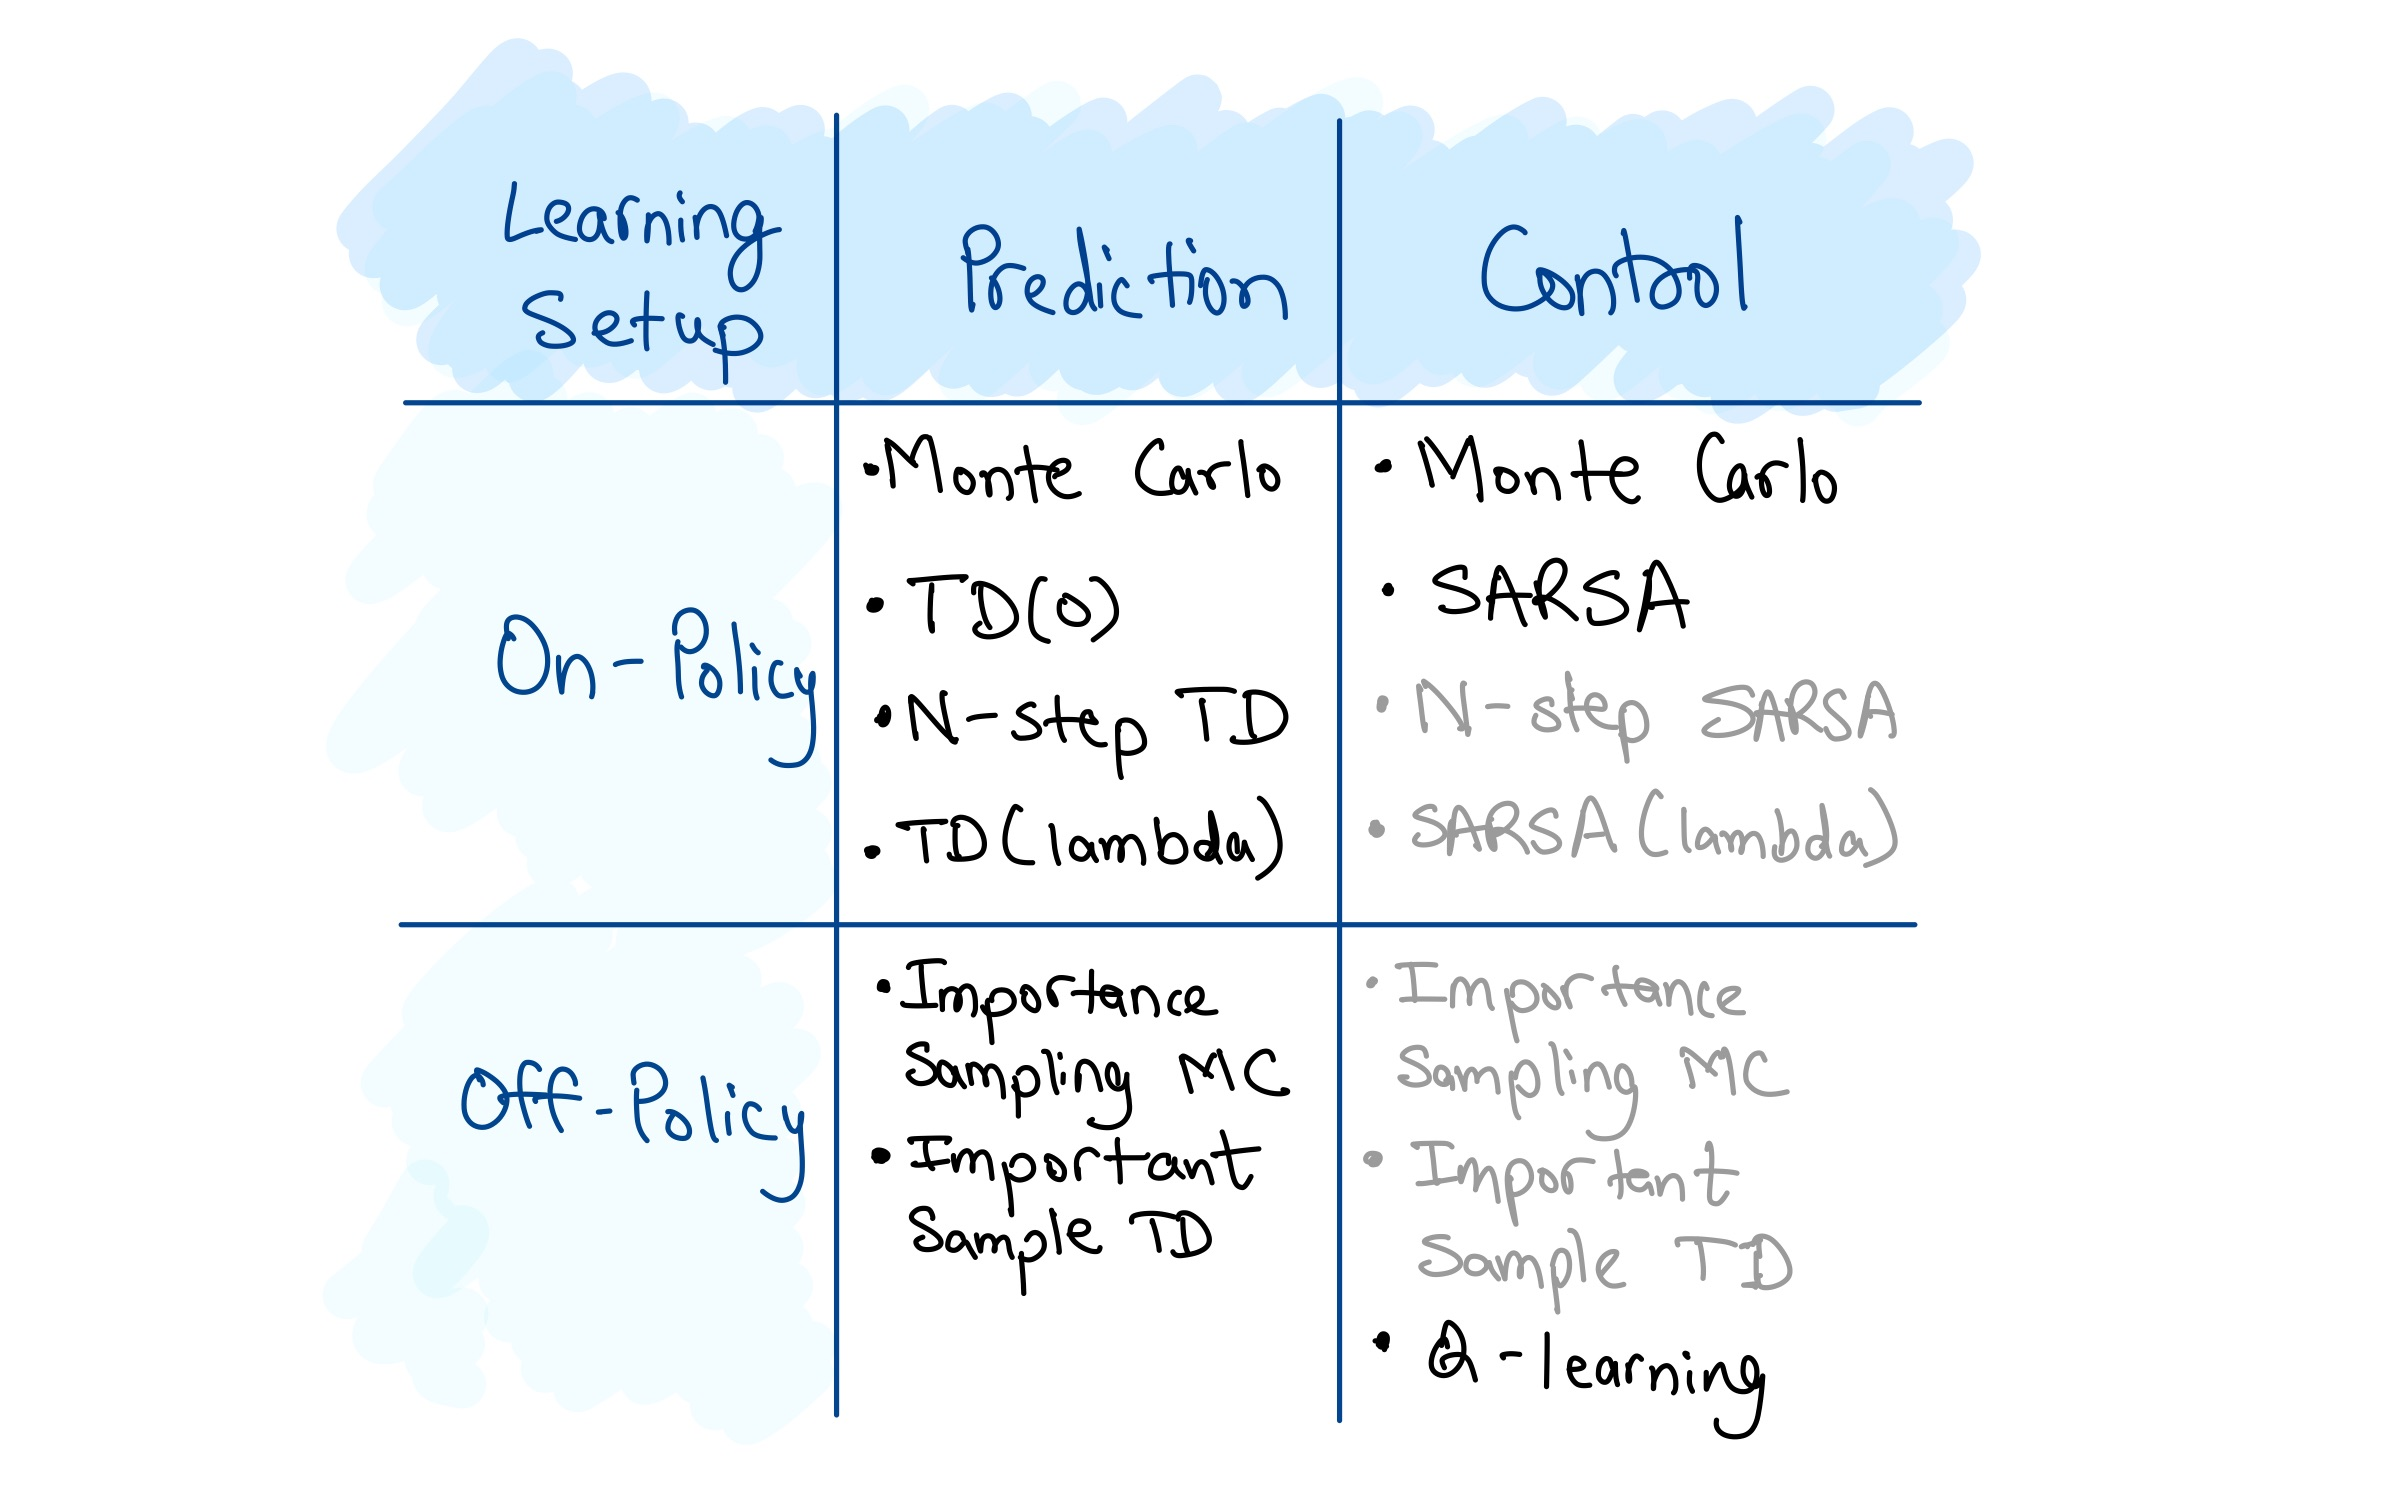
\includegraphics[width=0.7\textwidth]{model_free_classes.jpg}
    \caption{Classification of model-free value-based RL approaches taught in class (bold font)}
    \label{fig:model-free}
\end{figure}

\subsection{Value Function Approximation}

While learning the approaches in the previous section, it was assumed we have a finite state and action space, thus leading to a tabular value function. In a scenario where the state and action space is continuous and infinite, we use a function approximator to approximate the value function. These function approximators may be:

\begin{itemize}
    \item from continuous state space $s$ to value function $V_{\theta}(s)$.
    \item from continuous state space $s$ and action space $a$ to action-value function $Q_{\theta}(s,a)$. 
    \item from continuous state space $s$ to action-value function $Q_{\theta}(s,a_1)$, $Q_{\theta}(s,a_2)$, \ldots, $Q_{\theta}(s,a_M)$ for M discrete actions.

\end{itemize}

The function approximators can be of any architecture such as:

\begin{itemize}
    \item \textbf{Linear:} $V_{\theta}(s) = \theta^Tf(s)$ and $Q_{\theta}(s,a) = \theta^Tf(s,a)$ for handcrafted features $f(s)$ and $f(s,a)$.
    \item \textbf{NN:} $V_{\theta}(s) = NN_{\theta}(s)$ and $Q_{\theta}(s,a) = NN_{\theta}(s,a)$ for a neural network NN.
    \item \textbf{DNN:} $V_{\theta}(s) = DNN_{\theta}(s)$ and $Q_{\theta}(s,a) = DNN_{\theta}(s,a)$ for a deep neural network DNN.
\end{itemize}

\subsection{Value Function Approximation for Prediction}

The objective function to learn a function approximator for the value function is:
\begin{equation}
    \hat{\theta} = \arg \min\limits_\theta\mathbb{E}_p \left[(V(s) - V_{\theta}(s))^2 \right]
\end{equation}
The objective function can be optimized using online gradient descent where:
\begin{equation}
    \nabla_{\theta}J(\theta) \approx (V(s) - V_{\theta}(s)) \frac{\partial}{\partial \theta} V_{\theta}(s)
\end{equation}

where $V_{\theta}(s)$ is the function approximator and $V(s)$ is the true value function. Algorithm \ref{algo:vfap} highlights the steps of value function approximation for prediction. The true value function ($G^{(t)}$) can be obtained using any of the prediction methods in Fig. \ref{fig:model-free}.

\begin{algorithm}[H]
\caption{Approximate-Prediction(\pi, \alpha, V_{\theta})}
\label{algo:vfap}
\begin{algorithmic}[1]
\FOR{$e=1,\;\ldots,\;E$}

\STATE $\{s^{(t)}, a^{(t)}, r^{(t)}\}_{t=0}^T \sim \mathcal{E}|\pi$

\FOR{$t=0,\;\ldots,\;T$}
\STATE $\theta = \theta + \alpha \left( G^{(t)} - V_{\theta}(s^{(t)})\right)\frac{\partial}{\partial \theta}V_{\theta}(s^{(t)})$
\ENDFOR
\ENDFOR
\STATE $\textbf{return } V_{\theta}$
\end{algorithmic}
\end{algorithm}

\section{Summary}
In the class, we learned various algorithms for control in continuous spaces (Sec. \ref{sec:fac}). We then read about the basic paper introducing deep Q-learning (Sec. \ref{sec:dql}). We finally explored policy-based RL approaches (Sec. \ref{sec:policy}).

\subsection{Function Approximation for Control}
\label{sec:fac}

The methods learned for control in Fig. \ref{fig:model-free} can be reused for the continuous state space by doing the following:

\begin{itemize}
    \item Replace the value function parameter update with the Q function parameter update (use a function approximator in the process). 
    \item Do probabilistic behavior sampling instead of deterministic sampling since continuous state spaces require sampling. More specifically, select a random action with a probability of $\epsilon$ and select an action greedily with a probability of $1-\epsilon$.
\end{itemize}

\subsubsection{Monte-Carlo Control for Continuous Spaces}

Algorithm \ref{algo:mc-tabular} explains the tabular version of Monte-Carlo control.

\begin{algorithm}[H]
\caption{MC-Control-Tabular(\pi, \epsilon, \alpha)}
\label{algo:mc-tabular}
\begin{algorithmic}[1]
\FOR{$e=0,\;\ldots,\;E$}
\vspace{0.15cm}
\STATE $\{s^{(t)}, a^{(t)}, r^{(t)}\}_{t=0}^T \sim \mathcal{E}|\pi$
\vspace{0.15cm}
\FOR{$t=0,\;\ldots,\;T$}
\vspace{0.15cm}
\STATE $G^{(t)} = \sum\limits_{i=t}^T r^{(i)}$\\
\vspace{0.15cm}
\STATE $Q(a^{(t)}, s^{(t)}) = Q(a^{(t)}, s^{(t)}) + \alpha\left[ G^{(t)} - Q(a^{(t)}, s^{(t)})\right]$\\
\vspace{0.15cm}
\STATE $\pi(a|s) = \frac{\epsilon}{|\mathcal{A}|} + \mathbf{1}\left[ a = \arg \max\limits_a Q(a, s^{(t)})\right] (1-\epsilon)\;\; \forall a, s$
\vspace{0.15cm}
\ENDFOR
\ENDFOR
\STATE $\textbf{return } \pi$
\end{algorithmic}
\end{algorithm}

Line 5 in Algorithm \ref{algo:mc-tabular} is replaced with the function approximator update equation (line 6 in Algorithm \ref{algo:mc-continuous}) and line 6 in Algorithm \ref{algo:mc-tabular} is replaced with a probabilistic behavior sampling method (line 3 in Algorithm \ref{algo:mc-continuous}) to obtain the Monte-Carlo Control method for continuous action spaces.

\begin{algorithm}[H]
\caption{MC-Control-Continuous(\pi, \epsilon, \alpha)}
\label{algo:mc-continuous}
\begin{algorithmic}[1]
\FOR{$e=0,\;\ldots,\;E$}
\vspace{0.15cm}
\STATE $\pi \triangleq (1-\epsilon) \pi_{greedy} + (\epsilon)  \pi_{uniform}$
\vspace{0.15cm}
\STATE $\{s^{(t)}, a^{(t)}, r^{(t)}\}_{t=0}^T \sim \mathcal{E}|\pi$
\vspace{0.15cm}
\FOR{$t=0,\;\ldots,\;T$}
% \vspace{0.15cm}
\STATE $G^{(t)} = \sum\limits_{i=t}^T r^{(i)}$\\
\vspace{0.15cm}
\STATE $\theta = \theta + \alpha \left( G^{(t)} - Q_{\theta}(a^{(t)}, s^{(t)})\right)\frac{\partial}{\partial \theta}Q_{\theta}(a^{(t)}, s^{(t)})$
% \vspace{0.15cm}
\ENDFOR
\ENDFOR
\STATE $\textbf{return } \pi$
\end{algorithmic}
\end{algorithm}

\subsubsection{SARSA Control for Continuous Spaces}

Algorithm \ref{algo:sarsa-tabular} explains the tabular version of SARSA control.

\begin{algorithm}[H]
\caption{SARSA-Control-Tabular(\pi, \epsilon, \alpha)}
\label{algo:sarsa-tabular}
\begin{algorithmic}[1]
\FOR{$e=0,\;\ldots,\;E$}
\vspace{0.15cm}
\STATE $\{s^{(0)}, a^{(0)}\} \sim \mathcal{E}|\pi$
\vspace{0.15cm}
\FOR{$t=0,\;\ldots,\;T$}
\vspace{0.15cm}
\STATE $\{s^{(t)}, a^{(t)}, r^{(t)}, s^{(t+1)}, a^{(t+1)}\} \sim \mathcal{E}|\pi, s^{(t)}, a^{(t)}$
\vspace{0.15cm}

\STATE $G^{(t)} = r^{(t)} + \gamma Q(a^{(t+1)}, s^{(t+1)})$\\
\vspace{0.15cm}
\STATE $Q(a^{(t)}, s^{(t)}) = Q(a^{(t)}, s^{(t)}) + \alpha\left[ G^{(t)} - Q(a^{(t)}, s^{(t)})\right]$\\
\vspace{0.15cm}
\STATE $\pi(a|s) = \frac{\epsilon}{|\mathcal{A}|} + \mathbf{1}\left[ a = \arg \max\limits_a Q(a, s^{(t)})\right] (1-\epsilon)\;\; \forall a, s$
\vspace{0.15cm}
\ENDFOR
\ENDFOR
\STATE $\textbf{return } \pi$
\end{algorithmic}
\end{algorithm}


\begin{algorithm}[H]
\caption{SARSA-Control-Continuous(\pi, \epsilon, \alpha)}
\label{algo:sarsa-continuous}
\begin{algorithmic}[1]
\FOR{$e=0,\;\ldots,\;E$}
\vspace{0.15cm}
\STATE $\{s^{(0)}, a^{(0)}\} \sim \mathcal{E}|\pi$
\vspace{0.15cm}
\FOR{$t=0,\;\ldots,\;T$}
\vspace{0.15cm}
\STATE $\pi \triangleq (1-\epsilon) \pi_{greedy} + (\epsilon)  \pi_{uniform}$
\vspace{0.15cm}
\STATE $\{s^{(t)}, a^{(t)}, r^{(t)}, s^{(t+1)}, a^{(t+1)}\} \sim \mathcal{E}|\pi, s^{(t)}, a^{(t)}$
\vspace{0.15cm}

\STATE $G^{(t)} = r^{(t)} + \gamma Q_{\theta}(a^{(t+1)}, s^{(t+1)})$\\
\vspace{0.15cm}
\STATE $\theta = \theta + \alpha \left( G^{(t)} - Q_{\theta}(a^{(t)}, s^{(t)})\right)\frac{\partial}{\partial \theta}Q_{\theta}(a^{(t)}, s^{(t)})$
\vspace{0.15cm}
\ENDFOR
\ENDFOR
\STATE $\textbf{return } \pi$
\end{algorithmic}
\end{algorithm}


Lines 5,6 in Algorithm \ref{algo:sarsa-tabular} are replaced with the function approximator update equation (lines 6,7 in Algorithm \ref{algo:sarsa-continuous}) and line 7 in Algorithm \ref{algo:sarsa-tabular} is replaced with a probabilistic behavior sampling method (line 4 in Algorithm \ref{algo:sarsa-continuous}) to obtain the SARSA Control method for continuous action spaces.

\subsubsection{Q-learning Control for Continuous Spaces}

Algorithm \ref{algo:ql-tabular} explains the tabular version of Q-learning control.

\begin{algorithm}[H]
\caption{Q-learning-Control-Tabular(\mu, \epsilon)}
\label{algo:ql-tabular}
\begin{algorithmic}[1]
\FOR{$e=0,\;\ldots,\;E$}

\STATE $s^{(0)} \sim \mathcal{E}|\mu$
\vspace{0.15cm}
\FOR{$t=0,\;\ldots,\;T$}
\vspace{0.15cm}
\STATE $\{s^{(t)}, a^{(t)}, r^{(t)}, s^{(t+1)}\} \sim \mathcal{E}|\mu, s^{(t)}$
\vspace{0.15cm}
\STATE $a^* = \pi(s^{(t+1)}) \triangleq \arg \max\limits_a Q(a, s^{(t+1)})$
\vspace{0.15cm}

\STATE $G^{(t)} = r^{(t)} + \gamma Q^{\pi}(a^{*}, s^{(t+1)})$\\
\vspace{0.15cm}
\STATE $Q^{\pi}(a^{(t)}, s^{(t)}) = Q^{\pi}(a^{(t)}, s^{(t)}) + \alpha\left[ G^{(t)} - Q^{\pi}(a^{(t)}, s^{(t)})\right]$\\
\vspace{0.15cm}
\STATE $\mu(a|s^{(t+1)}) = \frac{\epsilon}{|\mathcal{A}|} + \mathbf{1}\left[ a = \pi(s^{(t+1)})\right] (1-\epsilon)$
\vspace{0.15cm}
\ENDFOR
\ENDFOR
\STATE $\textbf{return } \pi$
\end{algorithmic}
\end{algorithm}

Lines 6,7 in Algorithm \ref{algo:ql-tabular} are replaced with the function approximator update equation (lines 7,8 in Algorithm \ref{algo:ql-continuous}) and line 8 in Algorithm \ref{algo:ql-tabular} is replaced with a probabilistic behavior sampling method (line 4 in Algorithm \ref{algo:ql-continuous}) to obtain the Q-learning Control method for continuous action spaces.

\begin{algorithm}[H]
\caption{Q-learning-Control-Continuous(\mu, \epsilon)}
\label{algo:ql-continuous}
\begin{algorithmic}[1]
\FOR{$e=0,\;\ldots,\;E$}

\STATE $s^{(0)} \sim \mathcal{E}|\mu$
\vspace{0.15cm}
\FOR{$t=0,\;\ldots,\;T$}
\vspace{0.15cm}
\STATE $\mu \triangleq (1-\epsilon) \pi_{greedy} + (\epsilon)  \pi_{uniform}$
\vspace{0.15cm}
\STATE $\{s^{(t)}, a^{(t)}, r^{(t)}, s^{(t+1)}\} \sim \mathcal{E}|\mu, s^{(t)}$
\vspace{0.15cm}
\STATE $a^* = \pi_{greedy}(s^{(t+1)}) \triangleq \arg \max\limits_a Q(a, s^{(t+1)})$
\vspace{0.15cm}

\STATE $G^{(t)} = r^{(t)} + \gamma Q_{\theta}(a^{*}, s^{(t+1)})$\\
\vspace{0.15cm}
\STATE $\theta = \theta + \alpha \left( G^{(t)} - Q_{\theta}(a^{(t)}, s^{(t)})\right)\frac{\partial}{\partial \theta}Q_{\theta}(a^{(t)}, s^{(t)})$
\vspace{0.15cm}
\vspace{0.15cm}
\ENDFOR
\ENDFOR
\STATE $\textbf{return } \pi$
\end{algorithmic}
\end{algorithm}

\subsection{Deep Q-learning}
\label{sec:dql}

Minh et. al. \cite{mnih2015human} successfully used a deep neural network as the function approximator for Q-learning (naming it Deep Q-learning) to play like professional human players in Atari games. The algorithm they used (Algorithm \ref{algo:dql}) resembles the continuous Q-learning control method learned in the previous section, albeit with a few additional hacks which proved to be the key points for its success. 

\begin{algorithm}[H]
\caption{Deep Q-learning with Experience Replay}
\label{algo:dql}
\begin{algorithmic}[1]
\vspace{0.15cm}
\STATE Initialize replay memory $D$ to capacity $N$
\vspace{0.15cm}

\STATE Initialize action-value function $Q$ with random weights $\theta$
\vspace{0.15cm}

\STATE Initialize target action-value function $\hat{Q}$ with weights $\theta^{-} = \theta$
\vspace{0.15cm}

\FOR{episode = $1,\;\ldots,\;M$}
\vspace{0.15cm}
\STATE Initialize sequence $s_1 = \{x_1 \}$ and preprocessed sequence $\phi_1 = \phi(s_1)$
\vspace{0.15cm}
\FOR{$t=1,\;\ldots,\;T$}
\vspace{0.15cm}
\STATE With probability $\epsilon$ select a random action $a_t$ otherwise select $a_t = \arg \max\limits_a Q(\phi(s_t), a; \theta)$
\vspace{0.15cm}
\STATE Execute action $a_t$ in emulator and observe reward $r_t$ and image $x_{t+1}$
\vspace{0.15cm}
\STATE Set $s_{t+1} = s_t, a_t, x_{t+1}$ and preprocess $\phi_{t+1} = \phi(s_{t+1})$
\vspace{0.15cm}
\STATE Store transition ($\phi_t, a_t, r_t, \phi_{t+1}$) in $D$
\vspace{0.15cm}
\STATE Sample random minibatch of transitions ($\phi_j, a_j, r_j, \phi_{j+1}$) from $D$
\vspace{0.15cm}

\STATE Set $y_j = \begin{cases}
r_j & \text{if episode terminates at step $j+1$}\\
r_j + \gamma \max\limits_{a'} \hat{Q}(\phi_{j+1}, a'; \theta^{-}) & \text{otherwise}
 \end{cases}$
\vspace{0.15cm}
\STATE Perform gradient descent step on $\left(y_j - Q(\phi_j, a_j; \theta)\right)^2$ with respect to the network parameters $\theta$
\vspace{0.15cm}
\STATE Every C steps reset $\hat{Q} = Q$
\vspace{0.15cm}
\ENDFOR
\vspace{0.15cm}
\ENDFOR
\vspace{0.15cm}
\STATE $\textbf{return } \pi$
\end{algorithmic}
\end{algorithm}

Here, $x$ is an image of the Atari game and $\phi(s)$ is a deterministic pre-processed feature of this image. The similarities between Algorithm \ref{algo:ql-continuous} and Algorithm \ref{algo:dql} are as follows:
\begin{itemize}
    \item Lines 1, 2, 3 of Algorithm \ref{algo:ql-continuous} correspond to lines 4, 5, 6 of Algorithm \ref{algo:dql}. 
    \item Line 4 of Algorithm \ref{algo:ql-continuous} corresponds to line 7 of Algorithm \ref{algo:dql}.
    \item Line 5 of Algorithm \ref{algo:ql-continuous} corresponds to lines 8, 9 of Algorithm \ref{algo:dql}.
    \item Lines 6, 7 of Algorithm \ref{algo:ql-continuous} corresponds to line 12 of Algorithm \ref{algo:dql}.
    \item Line 8 of Algorithm \ref{algo:ql-continuous} corresponds to line 13 of Algorithm \ref{algo:dql}.
\end{itemize}

The few additional hacks which proved to be the key points for the success of Algorithm \ref{algo:dql} are as follows:
\begin{itemize}
    \item \textbf{Replay Buffer:} A memory $D$ of capacity $N$ stores the previous $N$ observed transitions ($\phi_t, a_t, r_t, \phi_{t+1}$). While training, a random minibatch of transitions is sampled from $D$ to break correlation and increase stability of the algorithm. Lines 1, 10, 11 in Algorithm \ref{algo:dql} correspond to this modification.
    \item \textbf{Delayed Updates:} Instead of updating the target policy in each time step, it is updated every C steps to increase the stability of the algorithm as well as to ensure split behavior policy and target policy. Line 14 of Algorithm \ref{algo:dql} corresponds to this modification. 
\end{itemize}

Codebase for the above algorithm is explained in the Appendix (Sec. \ref{sec:code}). Regret analysis of RL algorithms is still an ongoing area of research and thus not discussed in class.

\subsection{Policy Gradient Methods}
\label{sec:policy}

\subsubsection{Objective of Policy Gradient Methods}
\normalfont
In contrast to value-based reinforcement learning, policy gradients aim to optimize the expected return without explicitly estimating a value function. Instead, it learns directly from the policy by maximizing the expected return of a learning policy. It maximizes the following objective:
\begin{align*}
    \hat{\theta} &= \arg \max\limits_{\theta} \mathbb{E}_{p_\theta(\zeta)}\left[\sum\limits_{t=0}^Tr^{(t)}\right] \\
    &= \arg\max\limits_{\theta} J(\theta)
\end{align*}
This expected return term can be written more explicitly as 
$$\mathbb{E}_{p_\theta(\zeta)}\left[\sum\limits_{t=0}^Tr^{(t)}\right] = \int_\theta p_\theta(\theta)r(\zeta)d\zeta $$
where $r(\zeta) = \sum\limits^{T}_{t=0} r^{(t)}$\\
Recall the following notations in the expected value term:
\begin{align*}
    & p_\theta(\zeta) = p(s^{(0)})\Pi_{t=0}^T\pi_\theta(a^{(t)}|s^{(t)})p(s^{(t+1)}|s^{(t)}, a^{(t)}) \\
    & \zeta  = \{s^{(0)}, a^{(0)}, s^{(1)}, a^{(1)}, ..., s^{(T)}, a^{(T)}\} \\
    & r^{(t)} \triangleq r(s^{(t+1)}, a^{(t)}, s^{(t)})
\end{align*}

\subsubsection{Gradient Descent Update}

By taking the linear approximation of this objective with L2 regularization, and then solving for $\theta$ which optimizes the Lagrangian, we achieve the gradient descent update for $\theta$:
$$\hat{\theta} = \arg\max\limits_{\theta}\Big\{\alpha(J(\theta^{'})+\langle\theta-\theta^{'}, \nabla_{\theta^{'}}J(\theta^{'})\rangle - \frac{1}{2}||\theta-\theta^{'}||^2)\Big\}$$
$$\nabla_\theta\{\alpha(J(\theta^{'})+\langle\theta-\theta^{'}, \nabla_{\theta^{'}}J(\theta^{'})\rangle - \frac{1}{2}||\theta-\theta^{'}||^2)\} = 0 $$
$$\alpha\nabla_{\theta^{'}}J(\theta^{'}) - \theta + \theta^{'} = 0$$
$$\theta \leftarrow \theta^{'} + \alpha \nabla_{\theta^{'}}J(\theta^{'})$$

\subsubsection{Policy Gradient Derivation}

We now compute the $\nabla_{\theta^{'}}J(\theta^{'})$ term.
\begin{align*}
    \nabla_\theta J(\theta) &= \nabla_\theta \int_\zeta p_\theta(\zeta)r(\zeta)d\zeta \\ 
    &= \int_\zeta \nabla_\theta p_\theta(\zeta)r(\zeta)d\zeta \\
    &= \int_\zeta p_\theta(\zeta) \frac{\nabla_\theta p_\theta(\zeta)}{p_\theta(\zeta)}r(\zeta)d\zeta\\
    &= \int_\zeta p_\theta(\zeta) \nabla_\theta \ln p_\theta(\zeta)r(\zeta)d\zeta
\end{align*}
By expanding the natural log term, we will see that some terms that do not depend on $\theta$ can be eliminated from the gradient.
\begin{align*}
    \nabla_\theta \ln p_\theta(\theta) & = \nabla_\theta \left[ \ln p(s^{(0)}) + \sum_{t=1}^T \ln \pi_\theta(a^{(t)}|s^{(t)}) + \ln p(s^{(t+1)}|s^{(t)}, a^{(t)}) \right] \\
    & = \nabla_\theta \left[ \sum_{t=1}^T \ln \pi_\theta(a^{(t)}|s^{(t)})  \right] \\
    \nabla_\theta J(\theta) & = \int_\theta p_\theta \nabla_\theta \ln p_\theta(\theta)r(\zeta)d\zeta \\
    & = \int_\theta p_\theta \nabla_\theta \Bigg(\sum_{t=1}^T \ln \pi_\theta(a^{(t)}|s^{(t)})\Bigg) r(\zeta)d\zeta \\
    & = \mathbb{E}_{p_\theta}\left[ \Bigg( \sum_{t=1}^T \nabla_\theta \ln \pi_\theta(a^{(t)}|s^{(t)}) \Bigg) \Bigg( \sum_{t=1}^T r^{(t)} \Bigg) \right]
\end{align*}


% \section{Conclusion}

%\section*{References}
%Include your references here. Please cite any resources you found useful.	
%Populate the refs.bib file or list your references manually. Be consistent in formatting!
{
\bibliography{refs}
\bibliographystyle{abbrv}
}

\newpage
\section{Appendix}
%This section provides any relevant background material that was not covered in the lectures, but was found to be useful for understanding the material. 
%For example, derivations, theory underlying techniques employed, etc. 

%Additionally, this section can summarizes applications or extensions of these techniques found in the literature. 



\subsection{Example Code for Deep Q-learning}
\label{sec:code}

%New colors defined below
\definecolor{codegreen}{rgb}{0,0.6,0}
\definecolor{codegray}{rgb}{0.5,0.5,0.5}
\definecolor{codepurple}{rgb}{0.58,0,0.82}
\definecolor{backcolour}{rgb}{0.95,0.95,0.92}

%Code listing style named "mystyle"
\lstdefinestyle{mystyle}{
  backgroundcolor=\color{backcolour}, commentstyle=\color{codegreen},
  keywordstyle=\color{magenta},
  numberstyle=\tiny\color{codegray},
  stringstyle=\color{codepurple},
  basicstyle=\ttfamily\footnotesize,
  breakatwhitespace=false,         
  breaklines=true,                 
  captionpos=b,                    
  keepspaces=true,                 
  numbers=left,                    
  numbersep=5pt,                  
  showspaces=false,                
  showstringspaces=false,
  showtabs=false,                  
  tabsize=2
}

%"mystyle" code listing set
\lstset{style=mystyle}
\begin{lstlisting}[language=Python, caption=Deep Q-learning]
import numpy as np
import random
import gym
import tensorflow as tf
import keras

# Example Python code for training DQN corresponding to lines of Algorithm 8
def TrainDQN():
    # Line 1: Initialize replay buffer D to capacity N
    D = collections.deque(maxlen = N)
    # Line 2: Initialize action value function Q with random weights  
    Q = DQN()
    dqn.random_init()
    # Line 3: Initialize target action value function Q_hat with same weights
    Q_hat = DQN()
    Q_hat.weights = Q.weights
    # Line 4: for each episode...
    for i in range(M):
        # Line 5: Initialize sequence s1 and preprocessed sequence phi
        x = env.reset()
        s = [x]
        phi = preprocess(x)
        # Line 6: for each time step...
        for t in range(T):
            # Line 7: select random action or the action that maximizes Q
            q_values = dqn.predict(phi)
            if (random.random() < epsilon):
                a = np.random.choice(np.arange(q_values.shape[0]))
            else:
                a = np.argmax(q_values) 
            # Line 8: observe r and image x from action a
            next_x, r, done = env.step(a)
            # Line 9: set s_{t+1} and preprocess phi_{t+1}
            s.extend([a, next_x])
            next_phi = preprocess(next_s)
            # Line 10: store transition in replay memory
            D.append((phi, a, r, next_phi, done))
            # Line 11: Randomly sample minibatch of transitions
            transitions = random.sample(D, batch_size) 
            batch_phi = np.array([t[0] for t in transitions])
            batch_a = np.array([t[1] for t in transitions])
            batch_r = np.array([t[2] for t in transitions])
            batch_next_phi = np.array([t[3] for t in transitions])
            batch_done = [t[4] for t in transitions]
            # Line 12: set y_i
            batch_y = batch_r
            for i,done in enumerate(batch_done):
                if not done:
                    batch_y[i] += gamma*np.max(Q_hat.predict(batch_phi[i]))
            # Line 13: gradient descent on squared error with respect to theta
            DQN.backprop((batch_y - Q.predict(batch_phi)[batch_a])**2)
            # Line 14: copy weights every C steps
            if (t % C == 0): 
                Q_hat.weights = Q.weights
    # Line 17: return 
    return Q
\end{lstlisting}

\end{document} % Done!


